%%%%%%%%%%%%%%%%%%%%%%%%%%%%%%%%%%%%%%%%%
% Beamer Presentation
% LaTeX Template
% Version 2.0 (March 8, 2022)
%
% This template originates from:
% https://www.LaTeXTemplates.com
%
% Author:
% Vel (vel@latextemplates.com)
%
% License:
% CC BY-NC-SA 4.0 (https://creativecommons.org/licenses/by-nc-sa/4.0/)
%
%%%%%%%%%%%%%%%%%%%%%%%%%%%%%%%%%%%%%%%%%

%----------------------------------------------------------------------------------------
%	PACKAGES AND OTHER DOCUMENT CONFIGURATIONS
%----------------------------------------------------------------------------------------

\documentclass[
	11pt, % Set the default font size, options include: 8pt, 9pt, 10pt, 11pt, 12pt, 14pt, 17pt, 20pt
	%t, % Uncomment to vertically align all slide content to the top of the slide, rather than the default centered
	%aspectratio=169, % Uncomment to set the aspect ratio to a 16:9 ratio which matches the aspect ratio of 1080p and 4K screens and projectors
]{beamer}

\graphicspath{{fig/}{./}} % Specifies where to look for included images (trailing slash required)

\usepackage{booktabs} % Allows the use of \toprule, \midrule and \bottomrule for better rules in tables

%----------------------------------------------------------------------------------------
%	SELECT LAYOUT THEME
%----------------------------------------------------------------------------------------

% Beamer comes with a number of default layout themes which change the colors and layouts of slides. Below is a list of all themes available, uncomment each in turn to see what they look like.

%\usetheme{default}
%\usetheme{AnnArbor}
%\usetheme{Antibes}
%\usetheme{Bergen}
%\usetheme{Berkeley}
%\usetheme{Berlin}
%\usetheme{Boadilla}
%\usetheme{CambridgeUS}
%\usetheme{Copenhagen}
%\usetheme{Darmstadt}
%\usetheme{Dresden}
%\usetheme{Frankfurt}
%\usetheme{Goettingen}
%\usetheme{Hannover}
%\usetheme{Ilmenau}
%\usetheme{JuanLesPins}
%\usetheme{Luebeck}
\usetheme{Madrid}
%\usetheme{Malmoe}
%\usetheme{Marburg}
%\usetheme{Montpellier}
%\usetheme{PaloAlto}
%\usetheme{Pittsburgh}
%\usetheme{Rochester}
%\usetheme{Singapore}
%\usetheme{Szeged}
%\usetheme{Warsaw}

%----------------------------------------------------------------------------------------
%	SELECT COLOR THEME
%----------------------------------------------------------------------------------------

% Beamer comes with a number of color themes that can be applied to any layout theme to change its colors. Uncomment each of these in turn to see how they change the colors of your selected layout theme.

%\usecolortheme{albatross}
%\usecolortheme{beaver}
%\usecolortheme{beetle}
%\usecolortheme{crane}
%\usecolortheme{dolphin}
%\usecolortheme{dove}
%\usecolortheme{fly}
%\usecolortheme{lily}
%\usecolortheme{monarca}
%\usecolortheme{seagull}
\usecolortheme{seahorse}
%\usecolortheme{spruce}
%\usecolortheme{whale}
%\usecolortheme{wolverine}

%----------------------------------------------------------------------------------------
%	SELECT FONT THEME & FONTS
%----------------------------------------------------------------------------------------

% Beamer comes with several font themes to easily change the fonts used in various parts of the presentation. Review the comments beside each one to decide if you would like to use it. Note that additional options can be specified for several of these font themes, consult the beamer documentation for more information.

\usefonttheme{default} % Typeset using the default sans serif font
%\usefonttheme{serif} % Typeset using the default serif font (make sure a sans font isn't being set as the default font if you use this option!)
%\usefonttheme{structurebold} % Typeset important structure text (titles, headlines, footlines, sidebar, etc) in bold
%\usefonttheme{structureitalicserif} % Typeset important structure text (titles, headlines, footlines, sidebar, etc) in italic serif
%\usefonttheme{structuresmallcapsserif} % Typeset important structure text (titles, headlines, footlines, sidebar, etc) in small caps serif

%------------------------------------------------

%\usepackage{mathptmx} % Use the Times font for serif text
\usepackage{palatino} % Use the Palatino font for serif text

%\usepackage{helvet} % Use the Helvetica font for sans serif text
\usepackage[default]{opensans} % Use the Open Sans font for sans serif text
%\usepackage[default]{FiraSans} % Use the Fira Sans font for sans serif text
%\usepackage[default]{lato} % Use the Lato font for sans serif text

\usepackage{multicol}
\setlength{\columnsep}{0px}
\usepackage{{booktabs}}
\usepackage{graphicx}
\usepackage{subcaption}
\usepackage{xcolor,colortbl}
\usepackage{anyfontsize}


% -------------------------------------------------
% Cores
% -------------------------------------------------

% https://www.hexcolortool.com/F8E0E0#bded8c
\newcommand{\corTeoria}{f7b497}
\newcommand{\corExemplo}{8ce3ed}
\newcommand{\corExercicio}{e7e5e4}
\newcommand{\corNota}{ffce80}
\newcommand{\corCinza}{c5c9c6}
\newcommand{\corTodo}{9ee0ff}
\newcommand{\corCompetencia}{ADD8E6}
\newcommand{\corDefinicao}{FF7F50}

% https://www.colorhexa.com/ffb347
\newcommand{\corDestaque}{ffdca9}

% #####
% Cores do Brand book CLDF
% #####

% Cores da marca meio tom 
\definecolor{cldfA1}{RGB}{75, 87, 95} % Marrom 
\definecolor{cldfB1}{RGB}{246, 169, 36} % Laranja 
\definecolor{cldfC1}{RGB}{255, 229, 131} % Amarelo 

% Tabela Complementar
\definecolor{cldfA}{RGB}{228, 104, 11} % Laranjado
\definecolor{cldfB}{RGB}{240, 180, 80} % Amarelo
\definecolor{cldfC}{RGB}{0, 156, 218} % Azul Escuro
\definecolor{cldfD}{RGB}{89, 203, 232} % Azul Claro


\definecolor{cldfE}{RGB}{0, 144, 137} % Ciano Escuro
\definecolor{cldfF}{RGB}{110, 193, 182}  % Ciano Claro
\definecolor{cldfG}{RGB}{23, 163, 69} % Verde
\definecolor{cldfH}{RGB}{205, 205, 0} % Amarelo 

\definecolor{cldfK}{RGB}{228, 54, 137} % Rosa
\definecolor{cldfL}{RGB}{242, 168, 199} % Rosa Claro
\definecolor{cldfI}{RGB}{169, 57, 138} % Roxo
\definecolor{cldfJ}{RGB}{187, 150, 193} % Roxo Claro

% #####
% Tabelas do Texto
% #####
\definecolor{corMUST}{RGB}{228, 104, 11}
\definecolor{corSHOULD}{RGB}{240, 180, 80}
\definecolor{corCOULD}{RGB}{0, 156, 218}
\definecolor{corWOULD}{RGB}{187, 150, 193}

\definecolor{corP1}{RGB}{0, 144, 137} % Primeira Posicao
\definecolor{corP2}{RGB}{110, 193, 182} % Segunda Posicao
\definecolor{corP3}{RGB}{89, 203, 232} % Terceira Posicao
\definecolor{corPF}{RGB}{187, 150, 193} % Eliminados

\definecolor{corSIM}{RGB}{119, 221, 119} % Green
\definecolor{corNAO}{RGB}{255, 105, 97} % Red
\definecolor{corMED}{RGB}{253, 253, 150} % Amarelo


% #####
% Cores Adicionais
% #####


% https://colorhunt.co/palettes/pastel
% https://colorhunt.co/palette/ffb3b3ffdba4ffe9aec1efff
\definecolor{clPastelBlue}{HTML}{C1EFFF}
\definecolor{clPastelYellow}{HTML}{FFE9AE}
\definecolor{clPastelBrown}{HTML}{FFDBA4}
\definecolor{clPastelPink}{HTML}{FFB3B3}

% https://colorhunt.co/palettes/winter
% https://colorhunt.co/palette/002b5b2b4865256d858fe3cf
\definecolor{clWinterBlue1}{HTML}{8FE3CF}
\definecolor{clWinterBlue2}{HTML}{256D85}
\definecolor{clWinterBlue3}{HTML}{2B4865}
\definecolor{clWinterBlue4}{HTML}{002B5B}

% https://colorhunt.co/palettes/summer
% https://colorhunt.co/palette/fff5e4ffe3e1ffd1d1ff9494
\definecolor{clSummerRed1}{HTML}{FFF5E4}
\definecolor{clSummerRed2}{HTML}{FFE3E1}
\definecolor{clSummerRed3}{HTML}{FFD1D1}
\definecolor{clSummerRed4}{HTML}{FF9494}

% https://colorhunt.co/palette/eae5097dce135bb3182b7a0b
\definecolor{clNatureGreen1}{HTML}{EAE509}
\definecolor{clNatureGreen2}{HTML}{7DCE13}
\definecolor{clNatureGreen3}{HTML}{5BB318}
\definecolor{clNatureGreen4}{HTML}{2B7A0B}


% #####
% Cores Tabela Logs
% #####

\definecolor{clLogF}{HTML}{FFE9AE} % Amarelo
\definecolor{clLogA}{HTML}{7DCE13} % Verde
\definecolor{clLogB}{HTML}{FFD8A9} % Laranja
\definecolor{clLogC}{HTML}{FFB3B3} % Rosa
\definecolor{clLogD}{HTML}{FFF5E4} % Vermelho



%----------------------------------------------------------------------------------------
%	SELECT INNER THEME
%----------------------------------------------------------------------------------------

% Inner themes change the styling of internal slide elements, for example: bullet points, blocks, bibliography entries, title pages, theorems, etc. Uncomment each theme in turn to see what changes it makes to your presentation.

%\useinnertheme{default}
\useinnertheme{circles}
%\useinnertheme{rectangles}
%\useinnertheme{rounded}
%\useinnertheme{inmargin}

%----------------------------------------------------------------------------------------
%	SELECT OUTER THEME
%----------------------------------------------------------------------------------------

% Outer themes change the overall layout of slides, such as: header and footer lines, sidebars and slide titles. Uncomment each theme in turn to see what changes it makes to your presentation.

%\useoutertheme{default}
%\useoutertheme{infolines}
%\useoutertheme{miniframes}
%\useoutertheme{smoothbars}
%\useoutertheme{sidebar}
%\useoutertheme{split}
%\useoutertheme{shadow}
%\useoutertheme{tree}
%\useoutertheme{smoothtree}

%\setbeamertemplate{footline} % Uncomment this line to remove the footer line in all slides
%\setbeamertemplate{footline}[page number] % Uncomment this line to replace the footer line in all slides with a simple slide count

%\setbeamertemplate{navigation symbols}{} % Uncomment this line to remove the navigation symbols from the bottom of all slides

%----------------------------------------------------------------------------------------
%	PRESENTATION INFORMATION
%----------------------------------------------------------------------------------------

\title[\scalebox{.88}{\textsc{Intelligent Classification of Legislative Proposals}}]{Intelligent Classification of Legislative Proposals} % The short title in the optional parameter appears at the bottom of every slide, the full title in the main parameter is only on the title page

\subtitle{A Comparative Analysis of Machine Learning Models for Proposal Classification} % Presentation subtitle, remove this command if a subtitle isn't required

\author[Luca Peres \and Ronie Porfirio]{Luca Peres Quinta da Guarda \and Ronie Paulucio Porfirio} % Presenter name(s), the optional parameter can contain a shortened version to appear on the bottom of every slide, while the main parameter will appear on the title slide


\institute[UnB]{\textbf{Universidade de Brasília (UnB)} \\ \smallskip \textit{Programa de Pós-Graduação em Computação Aplicada}} % Your institution, the optional parameter can be used for the institution shorthand and will appear on the bottom of every slide after author names, while the required parameter is used on the title slide and can include your email address or additional information on separate lines

\date[20 de julho, 2024]{Course Mineração de Dados Massivos \\ \smallskip \scriptsize \textit{Prof. Dr. Marcelo Ladeira and Pr. MSc. Gustavo Cordeiro}} % Presentation date or conference/meeting name, the optional parameter can contain a shortened version to appear on the bottom of every slide, while the required parameter value is output to the title slide

%----------------------------------------------------------------------------------------

\begin{document}

%----------------------------------------------------------------------------------------
%	TITLE SLIDE
%----------------------------------------------------------------------------------------

\begin{frame}
	\titlepage % Output the title slide, automatically created using the text entered in the PRESENTATION INFORMATION block above
\end{frame}

%----------------------------------------------------------------------------------------
%	TABLE OF CONTENTS SLIDE
%----------------------------------------------------------------------------------------

% The table of contents outputs the sections and subsections that appear in your presentation, specified with the standard \section and \subsection commands. You may either display all sections and subsections on one slide with \tableofcontents, or display each section at a time on subsequent slides with \tableofcontents[pausesections]. The latter is useful if you want to step through each section and mention what you will discuss.

\begin{frame}
	\frametitle{Contents} % Slide title, remove this command for no title
	
	\tableofcontents % Output the table of contents (all sections on one slide)
	%\tableofcontents[pausesections] % Output the table of contents (break sections up across separate slides)
\end{frame}

%----------------------------------------------------------------------------------------
%	PRESENTATION BODY SLIDES
%----------------------------------------------------------------------------------------

% \section{Text Examples} % Sections are added in order to organize your presentation into discrete blocks, all sections and subsections are automatically output to the table of contents as an overview of the talk but NOT output in the presentation as separate slides

%------------------------------------------------

\subsection{Paragraphs and Lists}

\begin{frame}
	\frametitle{Paragraphs of Text}
	
	Sed iaculis \alert{dapibus gravida}. Morbi sed tortor erat, nec interdum arcu. Sed id lorem lectus. Quisque viverra augue id sem ornare non aliquam nibh tristique. Aenean in ligula nisl. Nulla sed tellus ipsum. Donec vestibulum ligula non lorem vulputate fermentum accumsan neque mollis.
	
	\bigskip % Vertical whitespace
	
	% Quote example
	\begin{quote}
		Sed diam enim, sagittis nec condimentum sit amet, ullamcorper sit amet libero. Aliquam vel dui orci, a porta odio.\\
		--- Someone, somewhere\ldots
	\end{quote}
	
	\bigskip % Vertical whitespace
	
	Nullam id suscipit ipsum. Aenean lobortis commodo sem, ut commodo leo gravida vitae. Pellentesque vehicula ante iaculis arcu pretium rutrum eget sit amet purus. Integer ornare nulla quis neque ultrices lobortis.
\end{frame}

%------------------------------------------------

\begin{frame}
	\frametitle{Lists}
	\framesubtitle{Bullet Points and Numbered Lists} % Optional subtitle
	
	\begin{itemize}
		\item Lorem ipsum dolor sit amet, consectetur adipiscing elit
		\item Aliquam blandit faucibus nisi, sit amet dapibus enim tempus
		\begin{itemize}
			\item Lorem ipsum dolor sit amet, consectetur adipiscing elit
			\item Nam cursus est eget velit posuere pellentesque
		\end{itemize}
		\item Nulla commodo, erat quis gravida posuere, elit lacus lobortis est, quis porttitor odio mauris at libero
	\end{itemize}
	
	\bigskip % Vertical whitespace
	
	\begin{enumerate}
		\item Nam cursus est eget velit posuere pellentesque
		\item Vestibulum faucibus velit a augue condimentum quis convallis nulla gravida 
	\end{enumerate}
\end{frame}

%------------------------------------------------

\subsection{Blocks}

\begin{frame}
	\frametitle{Blocks of Highlighted Text}
	
	\begin{block}{Block Title}
		Lorem ipsum dolor sit amet, consectetur adipiscing elit. Integer lectus nisl, ultricies in feugiat rutrum, porttitor sit amet augue.
	\end{block}
	
	\begin{exampleblock}{Example Block Title}
		Aliquam ut tortor mauris. Sed volutpat ante purus, quis accumsan.
	\end{exampleblock}
	
	\begin{alertblock}{Alert Block Title}
		Pellentesque sed tellus purus. Class aptent taciti sociosqu ad litora torquent per conubia nostra, per inceptos himenaeos.
	\end{alertblock}
	
	\begin{block}{} % Block without title
		Suspendisse tincidunt sagittis gravida. Curabitur condimentum, enim sed venenatis rutrum, ipsum neque consectetur orci.
	\end{block}
\end{frame}

%------------------------------------------------

\subsection{Columns}

\begin{frame}
	\frametitle{Multiple Columns}
	\framesubtitle{Subtitle} % Optional subtitle
	
	\begin{columns}[c] % The "c" option specifies centered vertical alignment while the "t" option is used for top vertical alignment
		\begin{column}{0.45\textwidth} % Left column width
			\textbf{Heading}
			\begin{enumerate}
				\item Statement
				\item Explanation
				\item Example
			\end{enumerate}
		\end{column}
		\begin{column}{0.5\textwidth} % Right column width
			Lorem ipsum dolor sit amet, consectetur adipiscing elit. Integer lectus nisl, ultricies in feugiat rutrum, porttitor sit amet augue. Aliquam ut tortor mauris. Sed volutpat ante purus, quis accumsan dolor.
		\end{column}
	\end{columns}
\end{frame}

%------------------------------------------------

\section{Table and Figure Examples}

\subsection{Table}

\begin{frame}
	\frametitle{Table}
	\framesubtitle{Subtitle} % Optional subtitle
	
	\begin{table}
		\begin{tabular}{l l l}
			\toprule
			\textbf{Treatments} & \textbf{Response 1} & \textbf{Response 2}\\
			\midrule
			Treatment 1 & 0.0003262 & 0.562 \\
			Treatment 2 & 0.0015681 & 0.910 \\
			Treatment 3 & 0.0009271 & 0.296 \\
			\bottomrule
		\end{tabular}
		\caption{Table caption}
	\end{table}
\end{frame}

%------------------------------------------------

\subsection{Figure}

\begin{frame}
	\frametitle{Figure}
	
	\begin{figure}
		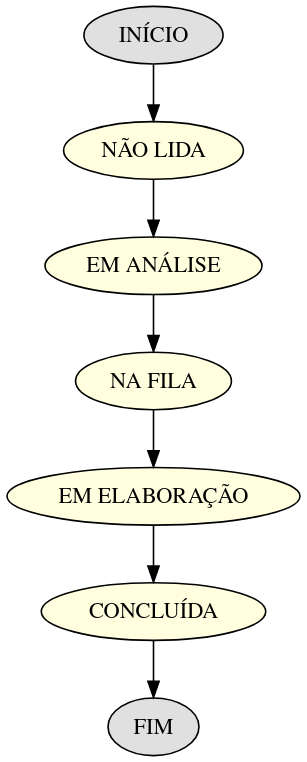
\includegraphics[width=0.2\linewidth]{fluxoBasico.png}
		\caption{Fluxo}
	\end{figure}
\end{frame}

%------------------------------------------------

\section{Mathematics}

\begin{frame}
	\frametitle{Definitions \& Examples}
	
	\begin{definition}
		A \alert{prime number} is a number that has exactly two divisors.
	\end{definition}
	
	\smallskip % Vertical whitespace
	
	\begin{example}
		\begin{itemize}
			\item 2 is prime (two divisors: 1 and 2).
			\item 3 is prime (two divisors: 1 and 3).
			\item 4 is not prime (\alert{three} divisors: 1, 2, and 4).
		\end{itemize}
	\end{example}
	
	\smallskip % Vertical whitespace
	
	You can also use the \texttt{theorem}, \texttt{lemma}, \texttt{proof} and \texttt{corollary} environments.
\end{frame}

%------------------------------------------------

\begin{frame}
	\frametitle{Theorem, Corollary \& Proof}
	
	\begin{theorem}[Mass--energy equivalence]
		$E = mc^2$
	\end{theorem}
	
	\begin{corollary}
		$x + y = y + x$
	\end{corollary}
	
	\begin{proof}
		$\omega + \phi = \epsilon$
	\end{proof}
\end{frame}

%------------------------------------------------

\begin{frame}
	\frametitle{Equation}

	\begin{equation}
		\cos^3 \theta =\frac{1}{4}\cos\theta+\frac{3}{4}\cos 3\theta
	\end{equation}
\end{frame}

%------------------------------------------------

\begin{frame}[fragile] % Need to use the fragile option when verbatim is used in the slide
	\frametitle{Verbatim}
	
	\begin{example}[Theorem Slide Code]
		\begin{verbatim}
			\begin{frame}
				\frametitle{Theorem}
				\begin{theorem}[Mass--energy equivalence]
					$E = mc^2$
				\end{theorem}
		\end{frame}\end{verbatim} % Must be on the same line
	\end{example}
\end{frame}

%------------------------------------------------

\begin{frame}
	Slide without title.
\end{frame}

%------------------------------------------------

\section{Referencing}

\begin{frame}
	\frametitle{Citing References}
	
	An example of the \texttt{\textbackslash cite} command to cite within the presentation:
	
	\bigskip % Vertical whitespace
	
	This statement requires citation \cite{p1,p2}.
\end{frame}

%------------------------------------------------

\begin{frame} % Use [allowframebreaks] to allow automatic splitting across slides if the content is too long
	\frametitle{References}
	
	\begin{thebibliography}{99} % Beamer does not support BibTeX so references must be inserted manually as below, you may need to use multiple columns and/or reduce the font size further if you have many references
		\footnotesize % Reduce the font size in the bibliography
		
		\bibitem[Smith, 2022]{p1}
			John Smith (2022)
			\newblock Publication title
			\newblock \emph{Journal Name} 12(3), 45 -- 678.
			
		\bibitem[Kennedy, 2023]{p2}
			Annabelle Kennedy (2023)
			\newblock Publication title
			\newblock \emph{Journal Name} 12(3), 45 -- 678.
	\end{thebibliography}
\end{frame}

%----------------------------------------------------------------------------------------
%	ACKNOWLEDGMENTS SLIDE
%----------------------------------------------------------------------------------------

\begin{frame}
	\frametitle{Acknowledgements}
	
	\begin{columns}[t] % The "c" option specifies centered vertical alignment while the "t" option is used for top vertical alignment
		\begin{column}{0.45\textwidth} % Left column width
			\textbf{Smith Lab}
			\begin{itemize}
				\item Alice Smith
				\item Devon Brown
			\end{itemize}
			\textbf{Cook Lab}
			\begin{itemize}
				\item Margaret
				\item Jennifer
				\item Yuan
			\end{itemize}
		\end{column}		
		\begin{column}{0.5\textwidth} % Right column width
			\textbf{Funding}
			\begin{itemize}
				\item British Royal Navy
				\item Norwegian Government
			\end{itemize}
		\end{column}
	\end{columns}
\end{frame}

%----------------------------------------------------------------------------------------
%	CLOSING SLIDE
%----------------------------------------------------------------------------------------

\begin{frame}[plain] % The optional argument 'plain' hides the headline and footline
	\begin{center}
		{\Huge The End}
		
		\bigskip\bigskip % Vertical whitespace
		
		{\LARGE Questions? Comments?}
	\end{center}
\end{frame}

%----------------------------------------------------------------------------------------


% =========================================================
\section{Introduction}
\begin{frame}
	\frametitle{Introduction}
	\framesubtitle{Business Understanding - Legislative Proposal's Definition and Types}

	\begin{exampleblock}{Legislative Proposal} 
	\begin{itemize}
		\item A \textbf{Legislative Proposal} is any matter subject to deliberation by the Legislative Chamber (CLDF Internal Regulations, art. 129).
	\end{itemize}
	\end{exampleblock}

	\begin{exampleblock}{} 
	\textbf{Legislative Proposals can be of the following types:}
	\begin{multicols}{2}
		\begin{itemize}
			\item Proposta de emenda à Lei Orgânica;
			
			\item Projeto de lei complementar;
			
			\item Projeto de lei;
			
			\item Projeto de decreto legislativo;
			
			\item Projeto de resolução;
			
			\item Indicação;
			
			\item Moção;
			
			\item Requerimento;
			
			\item Emenda;
			
			\item Recursos;
		\end{itemize}
	\end{multicols}
	\end{exampleblock}
\end{frame}
% --------------------------------------------------------------------------------------------
\begin{frame}
	\frametitle{Introduction}
	\framesubtitle{Business Understanding - Legislative Proposal's Themes}

	%https://ple.cl.df.gov.br/#/proposicao/buscar	
	\begin{exampleblock}{Legislative Proposals are classified into one or more themes:} 
		\begin{multicols}{3}
			\begin{itemize}
				\scriptsize
				\item Agricultura
				\item Assistência Social
				\item Assunto Fundiário e Ordenamento Territorial
				\item Assunto Social
				\item Cidadania
				\item Ciência e Tecnologia
				\item Combate à Corrupção
				\item Comunicação
				\item Comércio e Serviços
				\item Cultura
				\item Defesa do Consumidor
				\item Desenvolvimento Econômico
				\item Desporto e Lazer
				\item Direitos Humanos
				\item Economia
				\item Educação
				\item Energia
				\item Fiscalização e Governança
				\item Habitação
				\item Incentivos Fiscais e Concessões Públicas
				\item Indústria
				\item Meio Ambiente
				\item Não se aplica
				\item Outro
				\item Previdência Social
				\item Relações Exteriores
				\item Saneamento
				\item Saúde
				\item Segurança
				\item Servidor Público
				\item Trabalho
				\item Transporte e Mobilidade Urbana
				\item Turismo
				\item Urbanismo
				\normalsize
			\end{itemize}
		\end{multicols}
		\textbf{Total:} 34 themes	
	\end{exampleblock}
\end{frame}
% --------------------------------------------------------------------------------------------
\begin{frame}
	\frametitle{Introduction}
	\framesubtitle{Business Understanding - Why Themes?}
	\begin{block}{Thematic Classification Benefits} % Block without title
		\begin{itemize}
			\item Efficient classification of legislative proposals is crucial to \textbf{streamline their analysis} and processing within the legislative process helping to \textbf{determine which committees a proposal should go through}.
					
			% Otimizar a análise e o processamento dentro do processo legislativo, ajudando a determinar quais comissões uma proposta deve percorrer
					
			\item Thematic classification plays an important role in maintaining \textbf{accurate information retrieval} and \textbf{ensuring effective legislative management}.
			
			% Desempenha um papel importante na manutenção da recuperação precisa de informações e na garantia de uma gestão legislativa eficaz
			
			\item By categorizing legislative proposals into relevant themes, lawmakers can streamline their analysis, \textbf{allocate resources efficiently}, and \textbf{make informed decisions}. 
			
			% Alocar recursos de forma eficiente e tomar decisões informadas
				
			\item This process \textbf{enhances transparency} and facilitates a more \textbf{organized legislative workflow}.	
			% Melhora a transparência e facilita um fluxo legislativo mais organizado.
		\end{itemize}
	\end{block}
\end{frame}
% =========================================================
\section{The Problem}
\begin{frame}
	\frametitle{The Problem}
	\framesubtitle{Understanding the problem}
	\begin{alertblock}{Theme ``others'' is growing bigger}
		\begin{itemize}
			\item 	Usually, the author of the proposal is responsible for classifying it into one or more themes.
			
			% A escolha dos temas para classificação é feita pelo autor da proposição
			
			\item Unfortunately, due to various factors such as ambiguous topics, outdated categories, multidisciplinary nature, \textbf{many propositions end up being classified under the generic label of ``others''}.
			
			% Infelizmente, devido a diversos fatores, como tópicos ambíguos, categorias desatualizadas e natureza multidisciplinar, muitas proposições acabam sendo classificadas sob o rótulo genérico de “outros”.
			
		\end{itemize}
	\end{alertblock}	
\end{frame}
% --------------------------------------------------------------------------------------------
\begin{frame}
	\frametitle{The Problem}
	\framesubtitle{Understanding the problem}	
	\begin{figure}
		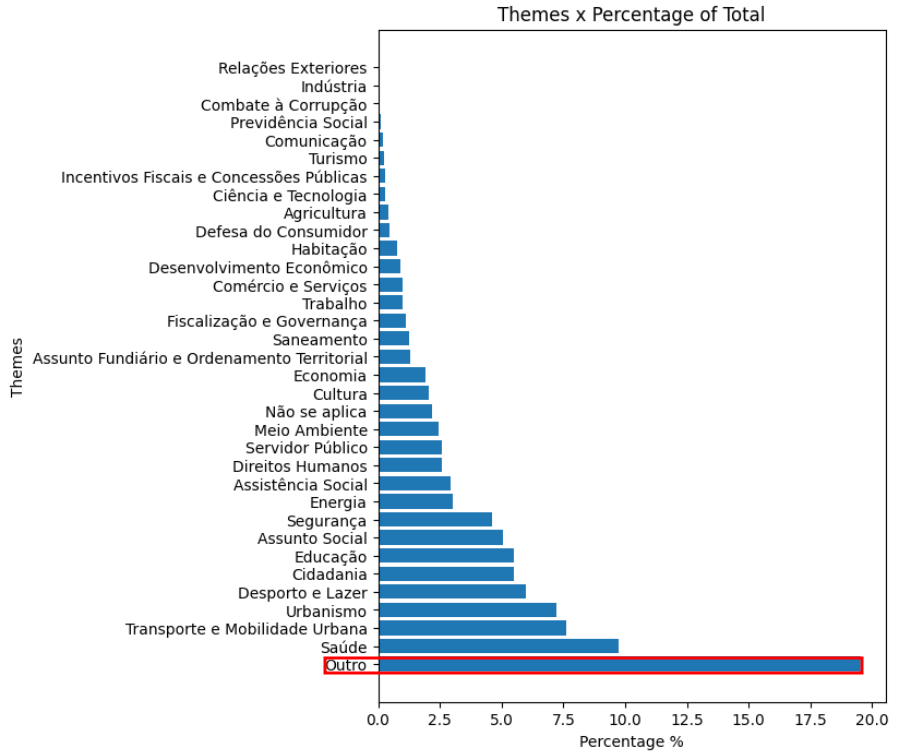
\includegraphics[width=0.6\linewidth]{graphThemes.png}
	\end{figure}

	\begin{block}{}
		\scriptsize
		The chart shows that the number of proposals classified under the theme “others” represents approximately 20\% of the total. 
	\end{block}	
\end{frame}
% --------------------------------------------------------------------------------------------
\begin{frame}
	\frametitle{The Problem}
	\framesubtitle{Problem definition}	

	\begin{alertblock}{The problem is inadequate proposal classification}
		Inadequate classification hinders efficient tracking, analysis, and transparency of legislative activities, making it difficult for both society and lawmakers to understand and oversee the legislative process effectively.
	\end{alertblock}	

	\begin{figure}
		
\includegraphics[width=0.3\linewidth]{problem.jpeg}
	\end{figure}


	% Essa classificação inadequada dificulta o acompanhamento eficiente, a análise e a transparência das atividades legislativas, tornando desafiador tanto para a sociedade quanto para os legisladores compreender e supervisionar efetivamente o processo legislativo. 
	
	

\end{frame}
% =========================================================
\section{Objective}
\begin{frame}
	\frametitle{Objective}
	
	\begin{block}{Objective} 
	\begin{itemize}
		\item The main goal is to create a model capable of sugesting new categorys for proposals classified under generic label ``others'' with themes that better suits that proposal.
	\end{itemize}
	\end{block}
		
	\begin{figure}
		
\includegraphics[width=0.3\linewidth]{arrow.jpeg}
	\end{figure}
		
	% O objetivo principal é criar um modelo capaz de sugerir novas categorias para propostas classificadas sob rótulo genérico ''outros'' com um ou mais temas que melhor se adaptem àquela proposta.
	
\end{frame}
% =========================================================
\section{Literature review}
\begin{frame}
	\frametitle{Literature review}
	
	Citar um ou dois artigos mais importantes.
	
	
\end{frame}
% =========================================================
\section{Methodology}
\begin{frame}
	\frametitle{Methodology}
	\begin{block}{CRISP-DM's Methodology} % Block without title
		\begin{enumerate}
			\item \textbf{Business Understanding}: We have analyzed legislative documents to align our data mining objectives with legislative classification needs.
			
			\item \textbf{Data Understanding}: The dataset comprises 22,267 summaries extracted from the Electronic Legislative Process (PLE) system, each accompanied by its respective thematic classification.
			
			\item \textbf{Data Preparation}: First, we discarded data classified under the 'Other' theme. Then, we performed tokenization, normalization, stopword removal, and lemmatization processes.
			
			\item (next slide)
		\end{enumerate}
	\end{block}
\end{frame}
% --------------------------------------------------------------------------------------------
\begin{frame}
	\frametitle{Methodology}
	\begin{block}{CRISP-DM's Methodology (cont...)} % Block without title
		\begin{enumerate}
			\setcounter{enumi}{3}
		
			\item \textbf{Modeling}: We use a multilingual sentence embedding model based on the MiniLM architecture, a lightweight and efficient BERT variant with 12 transformer layers, to produce high-quality embeddings for NLP tasks like semantic similarity, paraphrase identification and clustering.
			
			\item \textbf{Evaluation}: Our evaluation metrics include:
			\begin{enumerate}
				\item \textbf{Semantic Textual Similarity}: Pearson/Spearman correlation.
				
				\item \textbf{Paraphrase Identification}: Accuracy, F1 score, Precision, Recall.
				
				\item \textbf{Clustering}: Silhouette score, ARI, NMI.
			\end{enumerate}
	
			
			\item \textbf{Deployment}: The results will be used to create an interface in the PLE system to suggest themes that best fit new proposals.			
		\end{enumerate}
	\end{block}
\end{frame}
% =========================================================
\section{Experimentos Realizados}
\begin{frame}
	\frametitle{Experimentos Realizados}
	
	Falar do Embed
	
	
	
\end{frame}
% =========================================================
\section{Resultados}
\begin{frame}
	\frametitle{Resultados}
	
	
	
	
\end{frame}
% =========================================================
\section{Trabalhos Futuros}
\begin{frame}
	\frametitle{Resultados}
	
	
	
	
\end{frame}
% =========================================================
\section{Conclusões}
\begin{frame}
	\frametitle{Conclusões}
	
	
	
	
\end{frame}
% =========================================================






















% % =========================================================
\section{Módulos das Unidades da Assessoria Legislativa}
\begin{frame}
	\frametitle{Módulos das Unidades}
	
	\begin{alertblock}{Módulos das Unidades}
		\begin{itemize}
			\item \textbf{Módulo ``Gerenciar Solicitações da Unidade''}: Acessível por ambos perfis; 
			\item \textbf{Módulo ``Área de Trabalho do Consultor Legislativo''}: Cada Consultor acessa a sua própria área de trabalho;
			\item \textbf{Módulo ``Minhas Notificações''}: Cada usuário do sistema pode acessar sua própria tela de notificações;
		\end{itemize}
	\end{alertblock}	
\end{frame}
% =========================================================
\section{Módulo Gerenciar Solicitações das Unidades}

\begin{frame}
	\frametitle{Módulos das Unidades}
	\framesubtitle{Módulo Gerenciar Solicitações das Unidades}
	\begin{figure}
		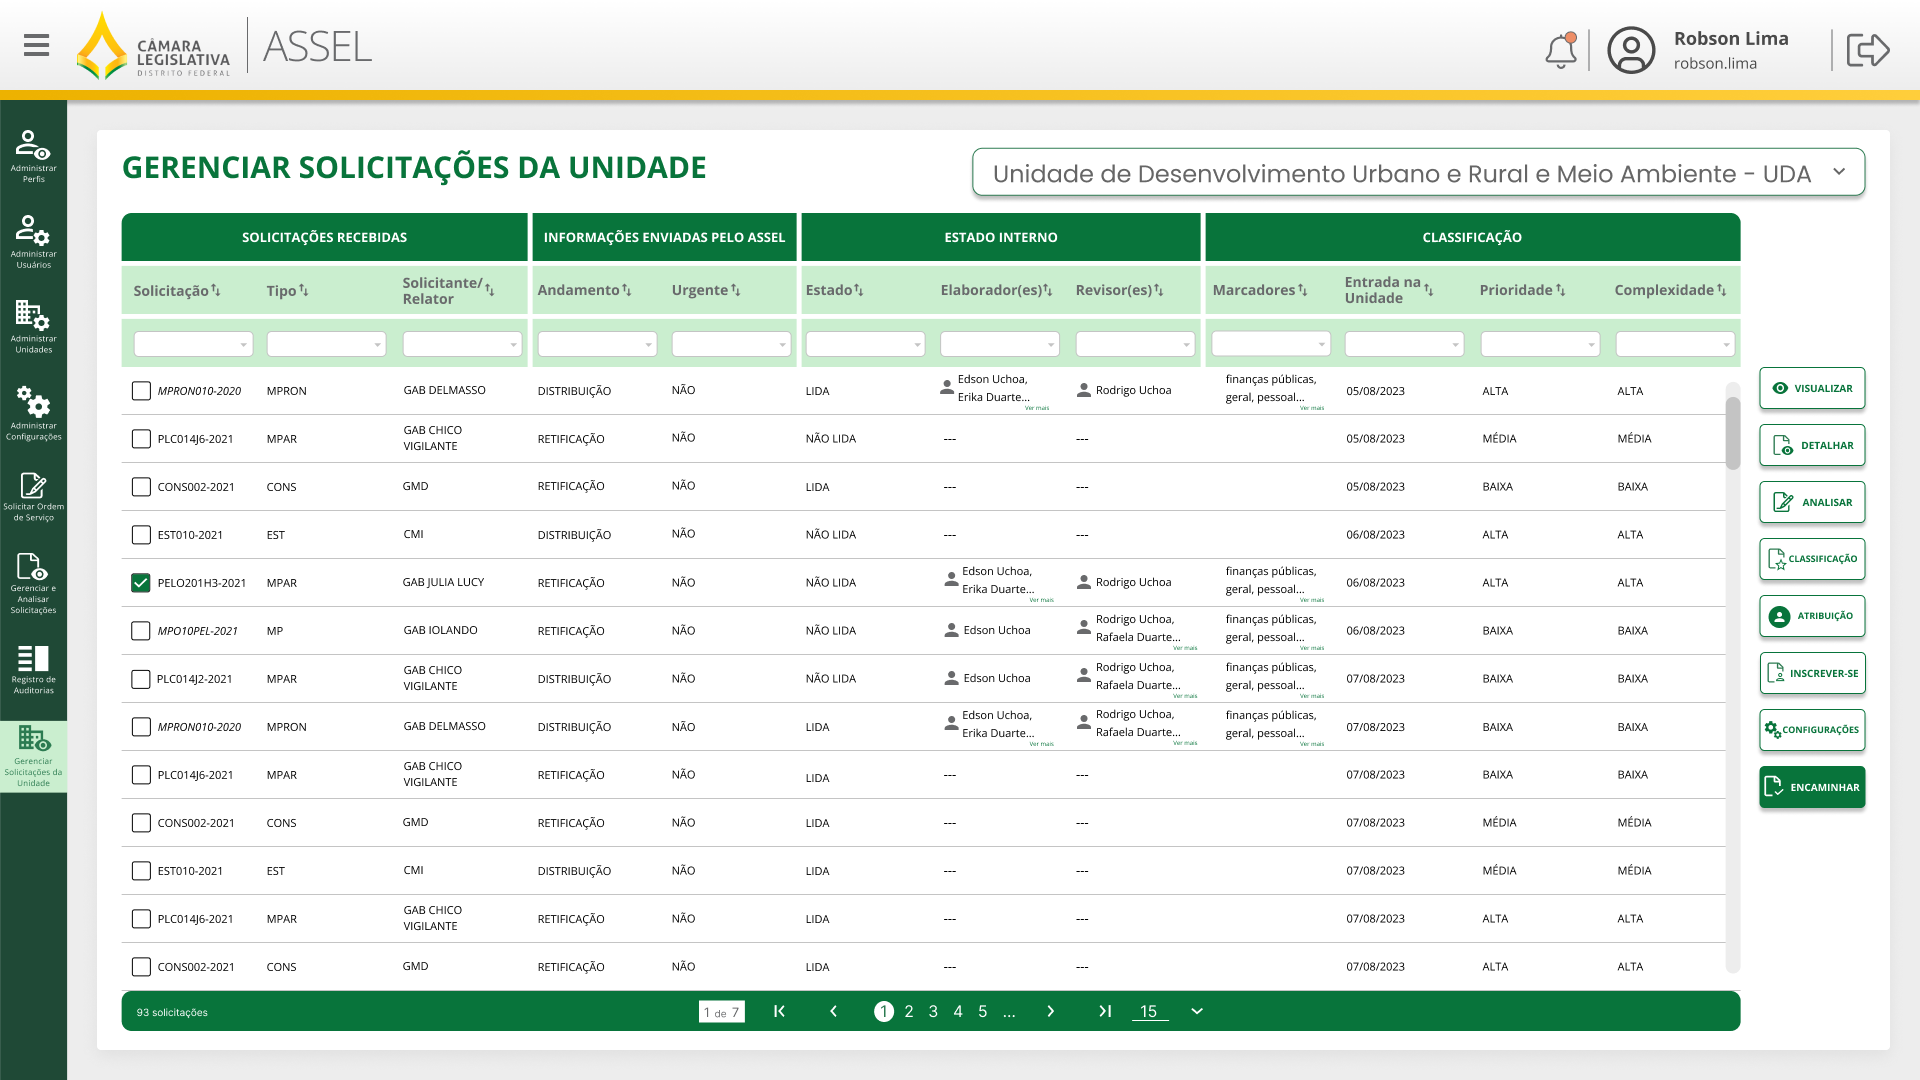
\includegraphics[width=0.99\linewidth]{GerSolUnid.png}
	\end{figure}
\end{frame}
% ------------------------------------------------------------
\begin{frame}
	\frametitle{Módulos das Unidades}
	\framesubtitle{Módulo Gerenciar Solicitações das Unidades - Objetivo}
	
	\begin{exampleblock}{Objetivo do ``Módulo Gerenciar Solicitações das Unidades''} 
		\begin{itemize}
			\item Gerenciamento pelos participantes da Unidade das solicitações que estão na carga de trabalho da Unidade.
		\end{itemize}
	\end{exampleblock}
\end{frame}
% ------------------------------------------------------------------
\begin{frame}
	\frametitle{Módulos das Unidades}
	\framesubtitle{Módulo Gerenciar Solicitações das Unidades}
	
	\begin{block}{Apresentação do Protótipo} % Block without title
		\begin{enumerate}
			\item Apresentar protótipo interativo do módulo;
			\item Explicar que cada Unidade da Assessoria Legislativa verá um módulo próprio e independente dos demais;
			\item Perfis:
			\begin{itemize}
				\item Supervisor
				\item Consultor Legislativo
			\end{itemize}
			
			\item Funcionalidades serão acessíveis de acordo com o perfil do usuário;
		\end{enumerate}
	\end{block}
\end{frame}
% =========================================================
\section{Módulo Área de Trabalho do Consultor Legislativo}

\begin{frame}
	\frametitle{Módulos das Unidades}
	\framesubtitle{Módulo Área de Trabalho do Consultor Legislativo}
	\begin{figure}
		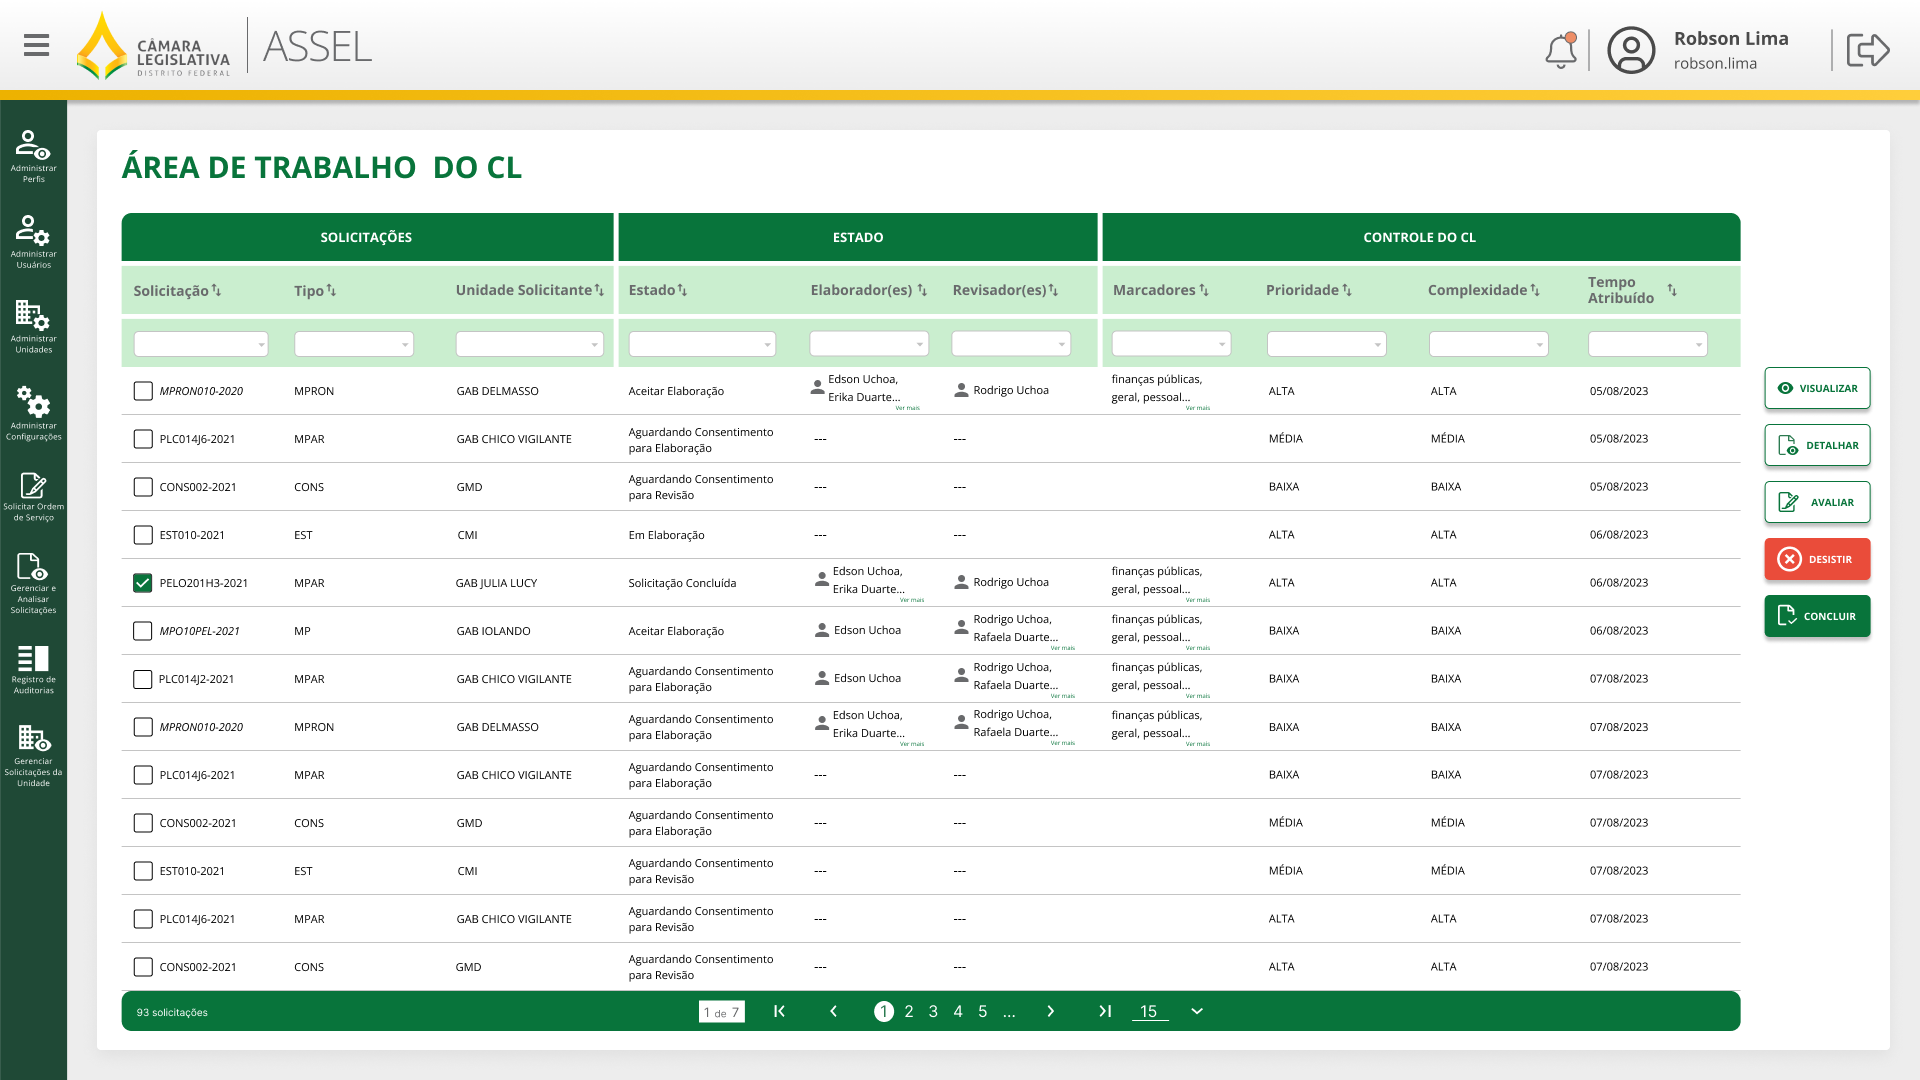
\includegraphics[width=0.99\linewidth]{AreaTrabalhoCL.png}
	\end{figure}
\end{frame}
% ------------------------------------------------------------
\begin{frame}
	\frametitle{Módulos das Unidades}
	\framesubtitle{Módulo Área de Trabalho do Consultor Legislativo - Objetivo}
	
	\begin{exampleblock}{Objetivos do Módulo ``Área de Trabalho do Consultor Legislativo''} 
		\begin{itemize}
			\item Gerenciamento pelo Consultor Legislativo da sua própria carga de trabalho na unidade;
			\item Gerenciamento de atividades de elaboração e revisão;
			\item Upload dos arquivos finais;
			\item Ferramentas:
			\begin{itemize}
				\item Relacionamentos entre solicitações;
				\item Acesso à consulta (a ser desenvolvida);
			\end{itemize}
			
		\end{itemize}
	\end{exampleblock}
\end{frame}
% =========================================================
\section{Módulo Minhas Notificações}

\begin{frame}
	\frametitle{Módulos das Unidades}
	\framesubtitle{Módulo Minhas Notificações}
	\begin{figure}
		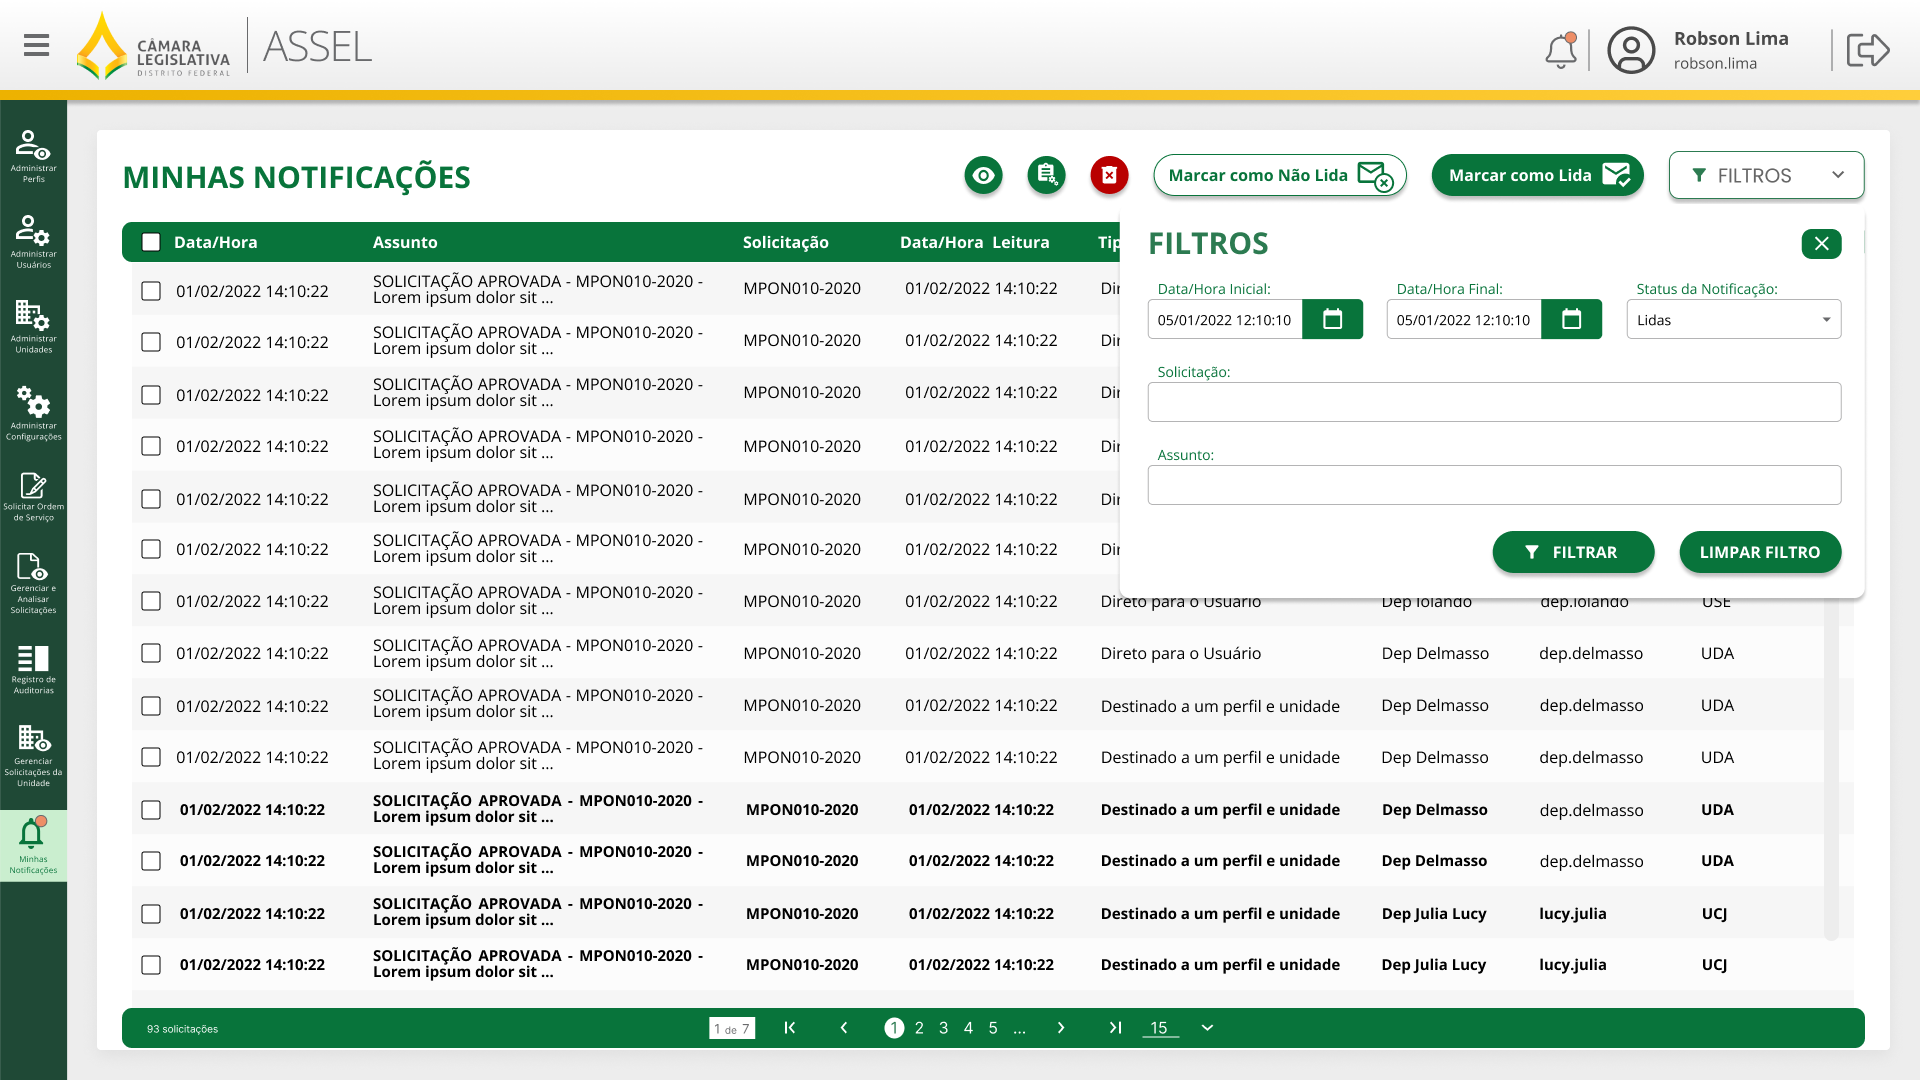
\includegraphics[width=0.99\linewidth]{MinhasNotificacoes.png}
	\end{figure}
\end{frame}
% ------------------------------------------------------------
\begin{frame}
	\frametitle{Módulos das Unidades}
	\framesubtitle{Módulo Minhas Notificações - Objetivo}
	
	\begin{exampleblock}{Objetivo} 
		\begin{itemize}
			\item Gerenciamento pelos usuários das notificações que receberam no sistema;
		\end{itemize}
	\end{exampleblock}
\end{frame}

% =========================================================

\section{Módulos das Unidades da Assessoria Legislativa}
\begin{frame}
	\frametitle{Módulos das Unidades}
	\framesubtitle{Observações}
	
	
	\begin{block}{Módulos das Unidades}
		\begin{itemize}
			\item Os três módulos funcionarão em conjunto;
			\item Permitir troca de informações entre os diversos atores de uma mesma Unidade de modo assíncrono:
			\begin{itemize}
				\item Teletrabalho;
			\end{itemize}
		\end{itemize}
	\end{block}	
\end{frame}
% =======================================


\section{Módulo Gerenciar Solicitações da Unidades - Funcionalidades}


\subsection{Visualizar, Detalhes e Classificação}

\begin{frame}
	\frametitle{Módulo Gerenciar Solicitações da Unidades}
	\framesubtitle{Funcionalidades}
	
	\textbf{Apresentação das Funcionalidades}
	
	\begin{alertblock}{Funcionalidades}
		\begin{enumerate}
			\item Funcionalidade ``Visualizar'';
			\item Funcionalidade ``Detalhes'';
			\item Funcionalidade ``Classificação'';
		\end{enumerate}
	\end{alertblock}	

	\begin{block}{} % Block without title
	\footnotesize Apresentar as funcionalidades usando a apresentação do protótipo. \normalsize
	\end{block}
	

\end{frame}



\begin{frame}
	\frametitle{Módulo Gerenciar Solicitações da Unidades}
	\framesubtitle{Estados Internos}

	\textbf{Estados Internos de uma Solicitação}

	\begin{figure}
		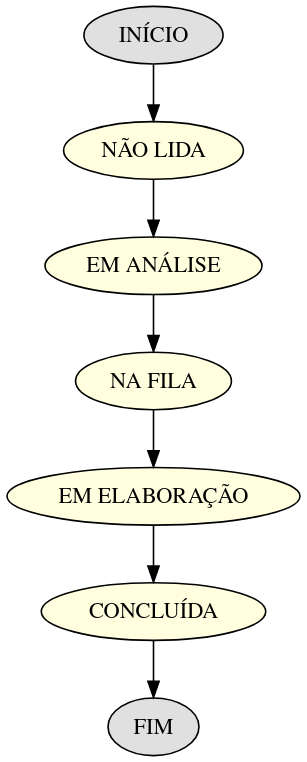
\includegraphics[width=0.2\linewidth]{fluxoBasico.png}
	\end{figure}
\end{frame}


\begin{frame}
	\frametitle{Módulo Gerenciar Solicitações da Unidades}
	\framesubtitle{Estados Internos}
	\begin{itemize}
		\item \textbf{Estado ``Não Lida''};
		\begin{itemize}
			\item Unidade ASSEL envia a solicitação para a Unidade fazendo-a aparecer na tabela de solicitações.
		\end{itemize}
	
		\item \textbf{Estado ``Em Análise''};
		\begin{itemize}
			\item Supervisor da Unidade seleciona a Solicitação e clica em ``Visualizar'' ou em ``Gerenciar Atribuições'' ou ainda em ``Analisar''.
		\end{itemize}
	
		\item \textbf{Estado: ``Na Fila''};
		\begin{itemize}
			\item Solicitações no estado ``Na Fila'' estão aguardando a alocação de Consultores;

			\item Se configurado, esse estado permite que os Consultores se inscrevam para atuarem como elaboradores.			
		\end{itemize}
	\end{itemize}
\end{frame}


\begin{frame}
	\frametitle{Módulo Gerenciar Solicitações da Unidades}
	\framesubtitle{Estados Internos - Em Elaboração}
	\begin{itemize}
		\item \textbf{Estado: ``Em Elaboração''};
		\begin{itemize}
			\item O estado ``Em Elaboração'' informa que uma dada solicitação está sendo desenvolvida por um ou mais Consultores. 
		\end{itemize}
	\end{itemize}

	\begin{block}{Elaboração e Revisão}
		\begin{itemize}
			\item A \textbf{Revisão} é uma atividade que acontece dentro do estado \textbf{``Em Elaboração''}.
			\item Isso permite manter a flexibilidades das diversas dinâmicas de elaboração e revisão dos trabalhos atualmente praticadas por cada unidade.
		\end{itemize}
	\end{block}
\end{frame}

\begin{frame}
	\frametitle{Módulo Gerenciar Solicitações da Unidades}
	\framesubtitle{Estados Internos - Estado Conclusão}
	\begin{itemize}
		\item \textbf{Estado: ``Conclusão''};
		\begin{itemize}
			\item Solicitações no estado ``Conclusão da Solicitação'' são elegíveis para serem encaminhados de volta para a ASSEL pelo Supervisor da Unidade. 
		\end{itemize}
	\end{itemize}
\end{frame}

\begin{frame}
	\frametitle{Módulo Gerenciar Solicitações da Unidades}
	\framesubtitle{Funcionalidades - Analisar}

	\textbf{Funcionalidade ``Analisar''}

	\begin{block}{Apresentação do Protótipo}
		\begin{itemize}
			\item Funcionalidade ``Analisar''
			\item Resultados:
			\begin{itemize}
				\item Aceitar e Colocar na Fila;
				\item Retorno (Devolução);
			\end{itemize}
		\end{itemize}
	\end{block}	
\end{frame}

\subsection{Distribuição Interna de Solicitações}

\begin{frame}
	\frametitle{Funcionalidades}
	\framesubtitle{Distribuição Interna de Solicitações}

	\textbf{Distribuição Interna de Solicitações}
	\begin{block}{Apresentação do Protótipo}
		\begin{itemize}
			\item ``Empurrar'' x  ``Puxar''
			\item Configurações
		\end{itemize}
	\end{block}	
\end{frame}


\begin{frame}
	\frametitle{Funcionalidades - Distribuição Interna de Solicitações}
	\framesubtitle{Empurrar x Puxar}

	\begin{itemize}
		\item \textbf{Empurrar = Atribuição pelo Supervisor}
		\item \textbf{Puxar = Inscrição pelo Consultor}
	\end{itemize}


		\begin{block}{Atribuição pelo Supervisor}
			\begin{itemize}
				\item Requer aceite ou rejeição pelo Consultor atribuído;
				\item Rejeição de atribuição pelo Consultor possui efeito imediato (não requer que o supervisor aceite ou recuse a rejeição);
			\end{itemize}
		\end{block}	


		\begin{block}{Inscrição pelo Consultor}
			\begin{itemize}
				\item Pode requerer Aprovação ou Recusa do Supervisor caso assim esteja configurado.
				
				\item Recusa de inscrição pelo Supervisor possui efeito imediato (não requer que o Consultor aceite ou rejeite a recusa);
			\end{itemize}
		\end{block}	



	\end{frame}



\subsection{Encaminhar}

\begin{frame}
	\frametitle{Funcionalidades}
	\framesubtitle{Encaminhar}
	
	\textbf{Encaminhamento de Solicitações Concluídas}
	
	\begin{block}{Apresentação do Protótipo}
		\begin{itemize}
			\item Encaminhar
		\end{itemize}
	\end{block}	

\end{frame}

\section{Próximos Passos}

\begin{frame}
	\frametitle{Próximos Passos}

	\begin{exampleblock}{Atualmente:}
		\begin{itemize}
			\item Módulo Gerenciar Solicitações das Unidades
			\item Módulo Área de Trabalho do CL
			\item Módulo de Minhas Notificações
		\end{itemize}
	\end{exampleblock}	

	\begin{block}{Para colocar em produção:}
		\begin{itemize}
			\item Módulo de Consulta
			\item Migração de Dados 
		\end{itemize}
	\end{block}	

	\begin{alertblock}{Futuro}
		\begin{itemize}
			\item Estatísticas e métricas de desempenho
			\item IA e BI
		\end{itemize}
	\end{alertblock}	
\end{frame}



\section{Feedback}

\begin{frame}
	\frametitle{Feedback}

	\begin{itemize}
		\item Feedback
	\end{itemize}
\end{frame}



\end{document} 
